% ======================================================================
% Post-Quantum Signature Verification for STARK-Based Smart Contracts
% IEEEtran Conference Style (2-column main, 1-column appendices)
% ======================================================================
% Build:
%   pdflatex main.tex
%   bibtex main   (optional; this file uses manual bibitems)
%   pdflatex main.tex
%   pdflatex main.tex
% ======================================================================

\documentclass[conference]{IEEEtran}

\usepackage[T1]{fontenc}
\usepackage{lmodern}
\usepackage{microtype}

\usepackage{amsmath,amssymb,amsfonts}
\usepackage{amsthm}

\usepackage{hyperref}
\usepackage{cite}

\usepackage{graphicx}
\usepackage{xcolor}

\usepackage{listings}
\lstset{
  basicstyle=\ttfamily\footnotesize,
  columns=fullflexible,
  breaklines=true,
  frame=single,
  xleftmargin=0.3em,
  xrightmargin=0.3em
}

\usepackage{tikz}
\usepackage{tikz-cd}
\usetikzlibrary{arrows.meta,positioning,shapes,calc}

% ---------------------------
% Theorem environments
% ---------------------------
\theoremstyle{definition}
\newtheorem{definition}{Definition}
\newtheorem{assumption}{Assumption}

\theoremstyle{plain}
\newtheorem{theorem}{Theorem}
\newtheorem{lemma}{Lemma}

\theoremstyle{remark}
\newtheorem{remark}{Remark}

% ---------------------------
% Macros
% ---------------------------
\newcommand{\F}{\mathbb{F}}
\newcommand{\B}{\mathbb{B}}
\newcommand{\bits}{\{0,1\}}
\newcommand{\negl}{\mathrm{negl}}
\newcommand{\concat}{\mathbin{\|}}

\newcommand{\Verify}{\mathrm{Verify}}
\newcommand{\Commit}{\mathrm{Commit}}
\newcommand{\Merkle}{\mathrm{Merkle}}
\newcommand{\Root}{\mathrm{Root}}
\newcommand{\PathVerify}{\mathrm{PathVerify}}
\newcommand{\Hash}{\mathcal{H}}

\newcommand{\Exec}{\llbracket \mathrm{exec}\rrbracket}

% ======================================================================
\title{Post-Quantum Signature Verification for STARK-Based Smart Contracts:\\
A Formal, Modular, and Future-Proof Cryptographic Framework}

\author{
\IEEEauthorblockN{Mayckon Giovani}
\IEEEauthorblockA{Independent Researcher / Systems Engineer\\
Email: \texttt{replace@me.example}}
}

\begin{document}
\maketitle

% ======================================================================
\begin{abstract}
Smart contract ecosystems remain structurally dependent on elliptic-curve signatures for state authorization, a dependency that becomes brittle under a realistic long-horizon adversary with eventual quantum capability. This paper specifies a research-grade framework for post-quantum authorization in STARK-based execution environments, with a primary focus on deterministic smart contract languages such as Cairo. Our design is intentionally hash-centric: it treats conservative symmetric assumptions (collision and preimage resistance) as the stable substrate for archival security, and then engineers a modular verification stack composed of hash abstractions, Merkle commitment systems, hash-based signatures (OTS/WOTS+/XMSS-family), and proof-system alignment through arithmetization.
We provide a formal semantic model of authorization as guarded transitions, compositional security arguments, and a roadmap toward proof-carrying transactions and recursive verification. Appendices include a Coq-oriented specification skeleton, HyperLTL formulations of authorization hyperproperties, and an AIR-level (Algebraic Intermediate Representation) specification outline for STARK arithmetization. The result is a cryptographic infrastructure layer intended to be auditable, reproducible, and extensible as a long-term research and engineering program.
\end{abstract}

\begin{IEEEkeywords}
Post-Quantum Cryptography, STARK, Cairo, Hash-Based Signatures, Merkle Trees, Formal Semantics, Hyperproperties, AIR, Proof-Carrying Authorization
\end{IEEEkeywords}

% ======================================================================
\section{Introduction}
Blockchains hard-code time asymmetry: state is permanent, while cryptographic assumptions are not. A system that is ``secure under current assumptions'' is insufficient when ledger state must remain enforceable decades later. Contemporary authorization flows typically rely on ECDSA/EdDSA; yet Shor-type quantum adversaries can collapse discrete-log hardness in polynomial time. Even if large-scale quantum machines are delayed, the attack \emph{store now, forge later} is rational: an adversary records signatures today and attempts key recovery or forgery later.

In parallel, the ZK ecosystem increasingly shifts execution into proof systems. STARK-based rollups and proof-verified smart contract environments require that security-critical logic be arithmetizable, deterministic, and bounded. Unfortunately, most NIST-standardized PQC signature schemes (notably lattice constructions) are computationally hostile to STARK-friendly execution constraints: they rely on large polynomial arithmetic, sampling, and heavy integer operations.

This paper takes a different foundation: post-quantum authorization for STARK-based contracts should begin with hash-based constructions. Hash-based signatures align with proof systems because their core operations are hash evaluations and simple combinators. We then elevate this baseline into a long-horizon, modular infrastructure that supports: (i) succinct public key commitments (Merkle roots), (ii) deterministic on-chain verification, (iii) proof-carrying authorization as a scaling primitive, and (iv) formal semantics and hyperproperty-level constraints to prevent cross-trace failures such as replay, equivocation, or accidental key reuse.

\subsection*{Contributions}
\begin{itemize}
\item We define a modular architecture for post-quantum authorization in Cairo/STARK environments: hash layer, Merkle layer, signature layer, contract layer, and proof layer.
\item We provide a formal semantic model of authorization as guarded state transitions and state formal theorems for authorization soundness under explicit assumptions.
\item We propose a proof-system alignment strategy via AIR constraints, enabling verification logic to become a first-class arithmetizable component.
\item We provide specification appendices: a Coq skeleton, HyperLTL properties, an AIR outline, and category-theoretic diagrams clarifying compositional structure.
\end{itemize}

% ======================================================================
\section{Threat Model and Long-Horizon Security}
We model an adversary $\mathcal{A}_Q$ with eventual quantum capability. The adversary can observe all on-chain data at time $t_0$ and attempt to forge authorization data at time $t_1 \gg t_0$ when quantum capabilities exist. Our objective is \emph{archival authorization}: the ability to validate that a state transition was authorized even after classical asymmetric assumptions fail.

\begin{assumption}[Quantum-Aware Hash Security]
\label{assm:hash}
The hash function family $\Hash$ is collision resistant and second-preimage resistant against quantum adversaries up to the chosen security level. We explicitly acknowledge Grover-type quadratic speedups; therefore parameters must be sized accordingly.
\end{assumption}

\begin{remark}
This work does not claim unconditional security. It formalizes a pivot to conservative assumptions that are currently believed to remain hard under quantum capabilities (modulo quadratic speedups), and then engineers deterministic verification under those assumptions.
\end{remark}

% ======================================================================
\section{System Overview: Layered Architecture}
We treat the system as an infrastructure stack rather than a single contract. The layers are:

\textbf{(L1) Hash Layer:} an abstraction over STARK-friendly hash primitives (e.g., Poseidon/Pedersen/Rescue-family), providing uniform interfaces for commitments and tree nodes.

\textbf{(L2) Merkle Layer:} generic Merkle trees with parameterized depth and hash choice, supporting inclusion proofs and root commitments.

\textbf{(L3) Signature Layer:} hash-based signature schemes (Lamport OTS, WOTS+, XMSS-like) expressed in terms of (L1) and (L2), producing signatures that are verifiable under bounded execution.

\textbf{(L4) Contract Layer:} authorization as a guard on state transitions; message binding rules; replay protection; index consumption enforcement.

\textbf{(L5) Proof Layer:} arithmetization and AIR constraints that make verification logic compatible with STARK proof generation and potentially recursive validation pipelines.

\subsection*{Engineering discipline}
From the first commit, the project must enforce reproducible builds, strict linting/formatting, CI matrices, security scanning, containerized dev environments, and enterprise OSS hygiene (CONTRIBUTING, SECURITY, CODE\_OF\_CONDUCT, templates). This is not process theater: cryptographic infrastructure fails through ambiguity, drift, and non-reproducibility.

% ======================================================================
\section{Formal Model of Authorization}
We define a deterministic labeled transition system.

\begin{definition}[Transition System]
A contract execution system is a triple $(S, A, \rightarrow)$ where $S$ is a set of states, $A$ is a set of actions, and $\rightarrow \subseteq S \times A \times S$ is a transition relation.
\end{definition}

We treat each action $a \in A$ as a structured input that includes an application message $M$ and authorization data $\sigma$ (signature or proof). Let $R$ be the public commitment (e.g., Merkle root) stored in contract state or configuration.

\begin{definition}[Authorization Predicate]
\label{def:auth}
Let $\Verify(R,M,\sigma)\in\B$ be the authorization predicate. A transition $(s,a,s')$ is authorized iff $\Verify(R,M,\sigma)=\texttt{true}$.
\end{definition}

\begin{definition}[Guarded Semantics]
The transition relation is restricted by the guard:
\[
s \xrightarrow{(M,\sigma)} s' \quad \text{only if} \quad \Verify(R,M,\sigma)=\texttt{true}.
\]
\end{definition}

\subsection*{Message Binding and Domain Separation}
A central failure mode in smart contracts is signing the wrong object: inconsistent encoding, missing domain separation, or replay across domains. We define a canonical message hash:
\[
m \gets \Hash(\textsf{domain} \concat \textsf{chain\_id} \concat \textsf{contract\_addr} \concat \textsf{nonce} \concat \Hash(\textsf{calldata})).
\]
Only $m$ is fed to signature verification.

% ======================================================================
\section{Commitments and Merkle Verification}
To avoid storing large PQC public keys on-chain, public key material is committed via a Merkle root.

\begin{definition}[Merkle Commitment]
Let leaves be $L_0,\ldots,L_{N-1}$. The Merkle root is $R=\Root(L_0,\ldots,L_{N-1})$ computed by iterated hashing. An inclusion proof $\pi$ for leaf $L_i$ is a sequence of sibling nodes that reconstructs $R$.
\end{definition}

\begin{definition}[Path Verification]
$\PathVerify(R, L_i, \pi, i)=\texttt{true}$ iff reconstructing the path using $\pi$ yields $R$.
\end{definition}

Merkle commitments are used to commit to OTS/WOTS public elements and, more generally, to commit to authorization sets (keys, roles, or policy roots).

% ======================================================================
\section{Hash-Based Signatures in STARK Environments}
Hash-based signatures are chosen for proof compatibility and long-horizon assumptions. We treat OTS-family schemes as a base layer and build composable constructions above.

\subsection{Lamport OTS (Foundation)}
Lamport OTS produces a public key consisting of hashes of secret pairs and signs by revealing one secret per message bit. This yields very simple verification (hash and compare), but signatures are large.

\subsection{WOTS+ (Compression via Chains)}
WOTS+ replaces per-bit reveals with chained hashes controlled by a Winternitz parameter. In a STARK environment, WOTS+ is attractive because the verifier performs repeated hash iterations (chain steps), which are arithmetizable and bounded.

\subsection{XMSS-like Trees (Many-Time from One-Time)}
XMSS extends OTS into a many-time scheme by placing OTS keys at leaves of a Merkle tree. On-chain state must enforce index non-reuse (or monotonicity), turning operational discipline into an explicit contract invariant.

% ======================================================================
\section{Formal Theorems: Soundness and Safety}
We state framework-level results under explicit assumptions.

\begin{theorem}[Authorization Soundness]
\label{thm:soundness}
Assume:
(i) the commitment root $R$ is correctly computed from the committed public elements,
(ii) $\PathVerify$ is sound (no false positives),
(iii) the signature verification procedure is correct relative to the committed public elements,
(iv) the contract enforces index non-reuse for OTS-family schemes.
Then no unauthorized state transition is reachable, i.e.,
\[
\forall s,s',M,\sigma,\quad \left(s \xrightarrow{(M,\sigma)} s'\right)\Rightarrow \Verify(R,M,\sigma)=\texttt{true}.
\]
\end{theorem}

\begin{proof}[Proof sketch]
By guarded semantics, the only transition rule permits $(M,\sigma)$ if $\Verify$ returns true. The assumptions ensure that $\Verify=\texttt{true}$ corresponds to a valid inclusion proof and a valid signature under committed public data, and that OTS indices cannot be reused to create equivocation across accepted transitions.
\end{proof}

\begin{theorem}[One-Time Index Safety]
\label{thm:ots}
Assume an OTS scheme where revealing secrets for two distinct messages under the same index permits existential forgery. If the contract enforces a strict no-reuse invariant on index $idx$, then existential forgery via reuse is prevented in the on-chain execution domain.
\end{theorem}

\begin{proof}[Proof sketch]
The only strategy that leverages on-chain reuse is blocked by the contract invariant. Even if an operator reuses keys off-chain, the contract rejects the second transition deterministically because the index check fails.
\end{proof}

\begin{lemma}[Merkle Inclusion Soundness]
\label{lem:merkle}
If $\Hash$ is collision resistant, then producing a proof $\pi$ such that $\PathVerify(R,L_i,\pi,i)=\texttt{true}$ for an uncommitted leaf $L_i$ is computationally infeasible up to $\negl(\lambda)$.
\end{lemma}

\begin{proof}[Proof sketch]
A successful forgery implies constructing an alternative leaf/path yielding the same root, inducing either a collision in $\Hash$ or a second-preimage in the tree compression structure.
\end{proof}

% ======================================================================
\section{Hyperproperties: Cross-Trace Authorization Safety}
Single-trace safety is insufficient for many authorization bugs. Cross-trace properties (hyperproperties) capture failures where each execution looks correct in isolation but the system fails when comparing multiple executions (replay, equivocation, cross-domain validity, index reuse across sessions). We treat these as spec-level requirements and formalize representative templates in Appendix~\ref{app:hyperltl}.

% ======================================================================
\section{AIR-Level Arithmetization Strategy}
STARK systems require expressing verification as algebraic constraints over a trace. We outline AIR constraints for: (i) hashing constraints, (ii) Merkle path constraints, (iii) chain constraints for WOTS+, and (iv) bit/field decomposition constraints for message binding. We present a structured AIR outline in Appendix~\ref{app:air}. The guiding principle is: verification logic must be expressible as a low-degree constraint system with bounded trace length. The contract implementation and the AIR specification should align so that ``verify in Cairo'' and ``verify in AIR'' are two views of the same semantic object.

% ======================================================================
\section{Category-Theoretic and Coalgebraic Structure}
Category theory is used here as a precision tool to prevent architectural entanglement. The central engineering problem in cryptographic infrastructure is interface drift: small changes in one layer silently invalidate assumptions of another layer.

\subsection{Functorial pipeline}
We model layers as morphisms:
\[
\mathsf{Secret}\xrightarrow{H}\mathsf{Hash}\xrightarrow{M}\mathsf{Tree}\xrightarrow{C}\mathsf{Root}\xrightarrow{V}\B.
\]
This pins down which invariants must be preserved at each interface.

\subsection{Coalgebraic contracts}
We model the contract as a coalgebra:
\[
\gamma:S\to F(S),
\]
where $F$ captures observable behaviors. Authorization guards refine $\gamma$ to an authorized coalgebra. This supports bisimulation arguments: two contract versions are equivalent if they produce the same authorized traces.

We include diagrams in Appendix~\ref{app:cat}.

% ======================================================================
\section{Engineering Program: Repository, CI/CD, and Enterprise OSS}
This framework is intended to be long-lived infrastructure, not a prototype.

\subsection*{Repository layout (from day 1)}
\begin{lstlisting}
/
  cairo/        # Cairo contracts + libraries
  rust/         # reference model + test generators + tooling
  python/       # benchmarking + analysis + CI helpers
  spec/         # Coq/Lean, HyperLTL, AIR docs
  docs/         # design docs + threat models + guides
  tests/        # cross-language vectors + fuzz harnesses
  scripts/      # reproducible build scripts
  docker/       # Dockerfiles (multi-stage)
  .devcontainer/# VS Code / Codespaces
  .github/      # workflows, templates, policies
\end{lstlisting}

\subsection*{Minimal required workflows}
\textbf{CI (multi-OS):} build + test + lint across Linux/macOS/Windows and relevant toolchain versions.  
\textbf{Security:} CodeQL + dependency scanning + supply-chain checks.  
\textbf{Release:} semantic versioning + changelog generation + signed tags + deterministic artifacts.

\subsection*{Developer environment}
A multi-stage Docker build plus a devcontainer configuration must exist so a contributor runs the full suite in a controlled environment with one command.

% ======================================================================
\section{Limitations and Scope Boundaries}
We are explicit about limitations.

\textbf{Not all PQC is proof-friendly.} This framework prioritizes hash-based signatures for compatibility. Lattice schemes may be integrated later via proof-carrying approaches (verify off-chain, prove correctness, verify proof on-chain), but not as direct Cairo verifiers initially.

\textbf{OTS discipline is a protocol problem.} The contract can enforce non-reuse for indices it observes, but off-chain operational discipline and secure key generation remain required.

\textbf{Parameters matter.} Grover-type speedups imply larger security parameters. Any ``quantum-safe'' claim must be parameterized and conservative.

% ======================================================================
\section{Roadmap: Research-Grade Implementation Plan}
This is a months-long plan with continuous publication of technical notes.

\subsection*{Phase 0: Infrastructure baseline (Days 1--10)}
\begin{itemize}
\item Initialize repo layout + enterprise OSS files (LICENSE, SECURITY, CODE\_OF\_CONDUCT, CONTRIBUTING).
\item Add strict formatting/linting; enforce via git hooks and CI gating.
\item Add devcontainer + Docker multi-stage build.
\item Add CI matrix: build/test/lint across OS and toolchain versions.
\item Establish a reference test-vector format and deterministic golden tests.
\end{itemize}

\subsection*{Phase 1: Hash layer (Days 11--30)}
\begin{itemize}
\item Implement hash abstraction interfaces in Cairo and a Rust reference model.
\item Provide Poseidon/Pedersen implementations or bindings; define a uniform transcript format.
\item Benchmark hashing cost: steps, memory, calldata patterns.
\item Publish: ``Hash Abstraction for STARK Contracts'' note.
\end{itemize}

\subsection*{Phase 2: Merkle layer (Month 2)}
\begin{itemize}
\item Implement generic Merkle verification (parametric depth, hash choice).
\item Add proof compression experiments (calldata packing).
\item Add fuzz tests comparing Cairo and Rust verifiers.
\item Publish: ``Merkle Commitments as On-Chain PQC Public Keys'' note.
\end{itemize}

\subsection*{Phase 3: Lamport OTS (Month 3)}
\begin{itemize}
\item Implement Lamport OTS verification using Merkle-root commitment for 512 elements.
\item Enforce index consumption discipline on-chain.
\item Provide reference keygen/signing tool in Rust with deterministic test vectors.
\item Publish: ``Lamport OTS in Cairo: Costs, Constraints, and Pitfalls'' note.
\end{itemize}

\subsection*{Phase 4: WOTS+ (Months 4--5)}
\begin{itemize}
\item Implement WOTS+ chaining with configurable Winternitz parameters.
\item Define correctness tests and encoding rules.
\item Explore tradeoffs: signature size vs steps vs proof complexity.
\item Publish: ``WOTS+ as the Practical Core for STARK-Friendly PQ Authorization''.
\end{itemize}

\subsection*{Phase 5: XMSS-like (Months 6--7)}
\begin{itemize}
\item Construct XMSS-lite by Merkleizing OTS public keys; define index evolution rules.
\item Implement secure root update/rotation semantics for long-lived contracts.
\item Publish: ``Many-Time PQ Authorization with Deterministic Index Discipline''.
\end{itemize}

\subsection*{Phase 6: Contract primitives (Months 8--9)}
\begin{itemize}
\item PQ vault, PQ multisig, timelocked root upgrades.
\item Message binding (domain separation) as a shared library.
\item Publish: ``Quantum-Safe Treasury Control in STARK Contracts''.
\end{itemize}

\subsection*{Phase 7: Proof-carrying authorization (Months 10--12)}
\begin{itemize}
\item Design: signature verified off-chain, correctness proved, proof verified on-chain.
\item Provide AIR constraints that mirror verifier semantics.
\item Publish: ``Proof-Carrying Transactions for Post-Quantum Authorization''.
\end{itemize}

% ======================================================================
\section{Conclusion}
We presented a formal and engineering-complete blueprint for post-quantum authorization in STARK-based smart contract environments. The framework is modular and proof-aligned: it treats hash-based cryptography as the stable long-horizon substrate and builds a layered system that can be verified deterministically in Cairo while also being expressible as algebraic constraints for STARK proofs. The theorems, hyperproperty specifications, AIR outline, and formal spec skeletons are the scaffold required for cryptographic infrastructure intended to live beyond the lifespan of current asymmetric assumptions.

% ======================================================================
% Bibliography (self-contained). You can swap to BibTeX later.
% ======================================================================
\begin{thebibliography}{99}

\bibitem{nistpqc}
NIST, ``Post-Quantum Cryptography Standardization Project,'' \emph{NIST CSRC}. Available: \url{https://csrc.nist.gov/projects/post-quantum-cryptography}

\bibitem{poseidon}
L.~Grassi, D.~Kales, D.~Rechberger, A.~Roy, and M.~Schofnegger, ``Poseidon: A New Hash Function for Zero-Knowledge Proof Systems,'' 2019. (See also IACR ePrint variants.)

\bibitem{stark}
E.~Ben-Sasson et al., ``Scalable, Transparent, and Post-Quantum Secure Computational Integrity,'' foundational works on STARKs, 2018--.

\bibitem{xmssrfc}
A.~H\"ulsing, D.~Butin, S.~Gazdag, J.~Rijneveld, and A.~Mohaisen, ``XMSS: eXtended Merkle Signature Scheme,'' RFC 8391, 2018.

\bibitem{sphincs}
D.~J. Bernstein et al., ``SPHINCS+: Submission to NIST PQC,'' 2019--2022.

\bibitem{cairo}
StarkWare, ``Cairo and Starknet Documentation,'' available via official documentation portals.

\bibitem{hypertlt}
M.~Rabe and B.~Finkbeiner, ``HyperLTL: A Temporal Logic for Hyperproperties,'' in \emph{CSF}, 2014.

\end{thebibliography}

% ======================================================================
% APPENDICES
% IMPORTANT: switch to one-column to avoid broken listings / wide TikZ in IEEE 2-col.
% ======================================================================
\appendices
\onecolumn

% ----------------------------------------------------------------------
\section{Appendix A: Formal Specification Skeleton in Coq}
\label{app:coq}
This appendix provides a Coq-oriented skeleton that captures the specification shape. It is intentionally abstract: the purpose is to define interfaces, invariants, and theorems that the implementation must refine. A full mechanization expands these modules with concrete Merkle inclusion predicates and explicit refinement links between the Cairo verifier and the formal model.

\begin{lstlisting}[language=]
(* ============================================================
   Coq Specification Skeleton (high-level)
   ============================================================ *)

Module Type HASH.
  Parameter t : Type.        (* hash output type *)
  Parameter msg : Type.      (* message/input type *)
  Parameter hash : msg -> t.

  (* Security assumptions appear as axioms or imported models. *)
  Axiom collision_resistant :
    forall (m1 m2: msg), hash m1 = hash m2 -> m1 = m2.
End HASH.

Module Type MERKLE (H: HASH).
  Parameter leaf : Type.
  Parameter root : Type.
  Parameter proof : Type.
  Parameter index : Type.

  Parameter mk_leaf : H.t -> leaf.
  Parameter compute_root : list leaf -> root.
  Parameter verify_path : root -> leaf -> proof -> index -> bool.

  (* Soundness: if verify_path says true, then leaf is included. *)
  Axiom verify_sound :
    forall (R: root) (L: leaf) (pi: proof) (i: index),
      verify_path R L pi i = true ->
      True.
End MERKLE.

Module Type OTS (H: HASH) (M: MERKLE H).
  Parameter pk_commitment : Type.   (* e.g., Merkle root *)
  Parameter sig : Type.
  Parameter message : Type.

  Parameter verify : pk_commitment -> message -> sig -> bool.

  (* Extract index from signature; used for on-chain discipline. *)
  Parameter idx : sig -> M.index.

  Axiom verify_correct :
    forall (R: pk_commitment) (m: message) (s: sig),
      verify R m s = true -> True.
End OTS.

Module Type CONTRACT (H: HASH) (M: MERKLE H) (S: OTS H M).
  Parameter State : Type.
  Parameter Msg : Type.
  Parameter Sig : Type.
  Parameter Root : Type.

  Parameter Verify : Root -> Msg -> Sig -> bool.
  Parameter step : State -> Msg -> State.

  Definition exec (st: State) (R: Root) (m: Msg) (sg: Sig) : option State :=
    if Verify R m sg then Some (step st m) else None.

  Theorem authorization_sound :
    forall st R m sg st',
      exec st R m sg = Some st' ->
      Verify R m sg = true.
  Proof.
    intros. unfold exec in H0.
    destruct (Verify R m sg); inversion H0; auto.
  Qed.
End CONTRACT.
\end{lstlisting}

\subsection*{Mechanization path}
A full proof development proceeds by: (i) modeling Merkle inclusion as an inductive predicate, (ii) linking Cairo verification to spec verification via refinement, and (iii) proving that contract-level index discipline implies OTS safety (Theorem~\ref{thm:ots}) under explicit cryptographic assumptions.

% ----------------------------------------------------------------------
\section{Appendix B: HyperLTL Hyperproperties for Authorization Safety}
\label{app:hyperltl}
Hyperproperties express relations across traces. They are essential when each execution looks fine in isolation but the system fails when comparing multiple executions (replay, equivocation, cross-domain signatures, index reuse across sessions).

Below are representative HyperLTL-style templates. They serve as spec requirements and can be used to guide model checking and differential fuzzing.

\subsection*{H1: Index non-reuse across traces}
Informally: no two accepted transactions reuse the same OTS/XMSS index.
\[
\forall \pi_1.\forall \pi_2.\;
(\textsf{Accepted}_{\pi_1} \wedge \textsf{Accepted}_{\pi_2} \wedge
\textsf{Idx}_{\pi_1} = \textsf{Idx}_{\pi_2}) \Rightarrow \pi_1 = \pi_2.
\]

\subsection*{H2: Domain separation}
A signature valid in one domain must not be valid in another domain.
\[
\forall \pi_1.\forall \pi_2.\;
(\textsf{SigOk}_{\pi_1} \wedge \textsf{SameSig}_{\pi_1,\pi_2} \wedge
\textsf{Domain}_{\pi_1}\neq \textsf{Domain}_{\pi_2}) \Rightarrow \neg \textsf{SigOk}_{\pi_2}.
\]

\subsection*{H3: Replay protection}
Nonce uniqueness (or monotonicity) is enforced across traces:
\[
\forall \pi_1.\forall \pi_2.\;
(\textsf{Accepted}_{\pi_1}\wedge \textsf{Accepted}_{\pi_2}\wedge
\textsf{Nonce}_{\pi_1}=\textsf{Nonce}_{\pi_2}\wedge
\textsf{Msg}_{\pi_1}=\textsf{Msg}_{\pi_2}) \Rightarrow \pi_1=\pi_2.
\]

\subsection*{Practical note}
These properties can be checked on simplified models and then enforced operationally through: strict message binding, explicit nonces, and deterministic on-chain index consumption for OTS-family schemes.

% ----------------------------------------------------------------------
\section{Appendix C: AIR Formal Specification Outline (STARK Arithmetization)}
\label{app:air}
This appendix provides a structured outline of AIR constraints for arithmetizing verification. A concrete instantiation depends on the chosen hash (Poseidon/Pedersen) and proof system conventions, but the shape is stable.

\subsection*{Trace structure}
Let the execution trace be a sequence of rows $T[0],\dots,T[N-1]$ over field $\F_p$. Columns include:
\begin{itemize}
\item message transcript columns (domain-separated hash inputs),
\item hash state columns (sponge/permutation states),
\item Merkle path columns (sibling nodes + direction bits),
\item WOTS chain columns (step counters and intermediate hashes),
\item boolean selector columns (enable flags, direction bits).
\end{itemize}

\subsection*{Constraint families}

\textbf{C1: Booleanity.} For any bit column $b$:
\[
b(b-1)=0.
\]

\textbf{C2: Hash permutation.} If Poseidon is used, each round is constrained by polynomial relations linking state-before, round constants, S-box, MDS multiplication, and state-after. (The precise form depends on the Poseidon parameters and arithmetization strategy.)

\textbf{C3: Merkle step constraints.} For level $\ell$ with node $x_\ell$, sibling $s_\ell$, and direction bit $d_\ell$:
\[
x_{\ell+1} = \Hash(\textsf{DS} \concat ((1-d_\ell)\cdot(x_\ell,s_\ell) + d_\ell\cdot(s_\ell,x_\ell))).
\]
In practice, concatenation is implemented via a domain-separated hash of two field elements.

\textbf{C4: WOTS chain constraints.} For a chain element with step counter $k$:
\[
y_{k+1} = \Hash(\textsf{DS} \concat y_k),
\]
and constraints enforce that exactly the configured number of steps occur.

\textbf{C5: Boundary constraints.}
At trace start: initialize transcript and counters.
At trace end: enforce computed root equals committed root $R$ and the final accept flag is $1$ if and only if all constraints passed.

\subsection*{Soundness interface contract}
The AIR spec must align with the Cairo verifier:
\[
\Exec_{\textsf{Cairo}}(M,\sigma)\text{ accepts } \iff
\Exec_{\textsf{AIR}}(M,\sigma)\text{ has a satisfying trace.}
\]
This is a refinement obligation: the implementation must be proven (ideal) or differentially tested (minimum) to match AIR semantics.

% ----------------------------------------------------------------------
\section{Appendix D: Category-Theoretic and Coalgebraic Diagrams}
\label{app:cat}
These diagrams express the modular pipeline and the off-chain/on-chain separation in a form that is robust against interface drift.

\subsection*{D1: Commitment and verification pipeline}
\begin{center}
\begin{tikzcd}[column sep=huge,row sep=large]
\mathsf{Secret} \arrow[r, "H"] &
\mathsf{Hash} \arrow[r, "M"] &
\mathsf{Tree} \arrow[r, "C"] &
\mathsf{Root} \arrow[r, "V"] &
\mathbb{B}
\end{tikzcd}
\end{center}

\subsection*{D2: Off-chain proving vs on-chain verification (adjunction intuition)}
\begin{center}
\begin{tikzcd}[column sep=huge,row sep=large]
\mathbf{OffChain} \arrow[r, shift left=1.2ex, "F"] &
\mathbf{OnChain} \arrow[l, shift left=1.2ex, "G"]
\end{tikzcd}
\end{center}

\[
\mathrm{Hom}_{\mathbf{OnChain}}(F(x), y)\cong \mathrm{Hom}_{\mathbf{OffChain}}(x, G(y)).
\]

\subsection*{D3: Authorized coalgebra (guarded behavior refinement)}
\begin{center}
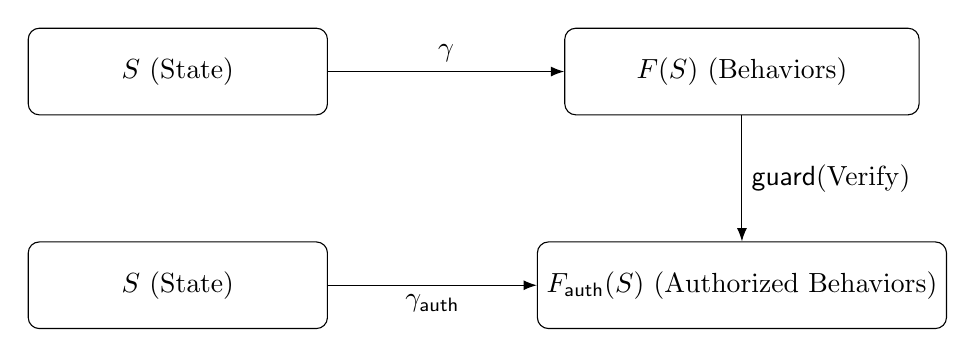
\begin{tikzpicture}[node distance=3.0cm,>=Latex]
\node[draw,rounded corners,minimum width=3.8cm,minimum height=1.1cm] (S) {$S$ (State)};
\node[draw,rounded corners,minimum width=4.5cm,minimum height=1.1cm,right=of S] (FS) {$F(S)$ (Behaviors)};
\draw[->] (S) -- node[above] {$\gamma$} (FS);

\node[draw,rounded corners,minimum width=5.0cm,minimum height=1.1cm,below=1.6cm of FS] (Fauth) {$F_{\textsf{auth}}(S)$ (Authorized Behaviors)};
\draw[->] (FS) -- node[right] {$\textsf{guard}(\Verify)$} (Fauth);

\node[draw,rounded corners,minimum width=3.8cm,minimum height=1.1cm,below=1.6cm of S] (S2) {$S$ (State)};
\draw[->] (S2) -- node[below] {$\gamma_{\textsf{auth}}$} (Fauth);
\end{tikzpicture}
\end{center}

\subsection*{Interpretation}
The contract’s raw behavior $\gamma$ is refined into authorized behavior $\gamma_{\textsf{auth}}$ by a guard induced by $\Verify$. This makes explicit a core design claim: authorization is a semantic restriction on the transition system, not an incidental conditional in code.

\end{document}